\documentclass[10pt,twocolumn,letterpaper]{article}

\usepackage{cvpr}
\usepackage{times}
\usepackage{epsfig}
\usepackage{graphicx}
\usepackage{amsmath}
\usepackage{amssymb}
\usepackage{booktabs}
\usepackage{microtype}
% From https://ctan.org/pkg/matlab-prettifier
\usepackage[numbered,framed]{matlab-prettifier}
\newcommand{\vect}[1]{\boldsymbol{\mathbf{#1}}}
\DeclareMathOperator*{\argmax}{arg\,max}
\DeclareMathOperator*{\argmin}{arg\,min}
\frenchspacing

\frenchspacing

% Include other packages here, before hyperref.

% If you comment hyperref and then uncomment it, you should delete
% egpaper.aux before re-running latex.  (Or just hit 'q' on the first latex
% run, let it finish, and you should be clear).
\usepackage[pagebackref=true,breaklinks=true,letterpaper=true,colorlinks,bookmarks=false]{hyperref}

\cvprfinalcopy % *** Uncomment this line for the final submission

\def\cvprPaperID{****} % *** Enter the CVPR Paper ID here
\def\httilde{\mbox{\tt\raisebox{-.5ex}{\symbol{126}}}}

% Pages are numbered in submission mode, and unnumbered in camera-ready
\ifcvprfinal\pagestyle{empty}\fi
\begin{document}

%%%%%%%%% TITLE
\title{SYDE 671 Final Project Report:\\
Unsupervised Visual Domain Adaptation: A Deep Max-Margin Gaussian Process Approach}

\author{JunYong Tong, Nick Torenvliet\\
University of Waterloo\\
\today
}

\maketitle
%\thispagestyle{empty}

%%%%%%%%% ABSTRACT
% [1430: James] We'll ignore the abstract for now.
\begin{abstract}
In this project we implement and adapt the Unsupervised Domain Adaptation(UDA) approach described in ~\cite{kim2019unsupervised}.

We begin with a brief description of the problem's context and introduce the various pieces of mathematical kit required to support the solution.  

We go on to provide the basis for an adaptation of the method proposed in ~\cite{kim2019unsupervised} by integrating the natural gradient method as given in ~\cite{khan2018fast}.  

We implement the approach in ~\cite{kim2019unsupervised}, as well as the natural gradient adaptation and then compare training outcomes of the two approaches across a grid of hyper-parameter selections.  An ensuing discussion of results identifies the improvement our adaptation provides.

Finally we discuss potential applications for Domain Adaptation.
\end{abstract}

%%%%%%%%% BODY TEXT
\section{Introduction}
In general deep learning requires well labelled training and test data that are independently and identically distributed (i.i.d). It is often difficult to meet the requirement for large labelled datasets, as the process of aquiring them can be time-consuming, costly, and laborious.   

UDA is the task of training a model on labelled data from a source distribution so that it performs well on unlabelled data from a target distribution with common labels.  Successful UDA application may provide good classification results while simultaneously reducing the burdensome requirement for labelled training data. 

A common example might be the training of a text sentiment analysis system to classify email from clients to lawyers as either satisfied or unsatisfied. 
Utilizing UDA you could attempt to perform training using a labeled set of email from clients to financial advisors, and an unlabelled set of emails from clients to lawyers.

\section{Related Work}

The original account of domain adaptation is provided by Ben-David in ~\cite{ben2010theory}, in which a theoretical upper-bound for error was provided. 

There are three main approaches to tackling the domain adaptation problem.

The marginal matching strategy focuses on transferring deep neural network representations from a labelled source dataset to an unlabelled target dataset by matching the distributions of features between different domains, to extract domain-invariant features \cite{sun2016deep}. 

Generative modeling methods, \cite{rebuffi2017learning} \cite{courty2017joint} \cite{benaim2017one}, leverage an adversarial training strategy which allows the learning of feature representations to be discriminative for the labelled source domain data and indistinguishable between source and target domains.

A third approach utilizes a shared latent space to learn an embedding that are used for classification in the target domain.  For example, \cite{liu2017unsupervised} proposed unsupervised image-to-image translation framework based on the \cite{liu2016coupled}.  

Kim et. al. in ~\cite{kim2019unsupervised} provide the latest in a genre of literature related to the problem of UDA via latent spaces.  Their adaptation, the subject of this paper, utilizes Gaussian processes and variational inference to further refine the latent space based UDA approach.  From this point on we use UDA to denote the method present in ~\cite{kim2019unsupervised}.     

\section{Unsupervised Domain Adaptation}
To formalize the notion of latent space based UDA, consider a joint space of inputs and class labels, \(\mathcal{X} \times \mathcal{Y}\) where \(\mathcal{Y} = \{1,\dots,K\}\). 

Consider a source \textbf{S} and target \textbf{T} domain on this space,  with unknown distributions \(p_S(\vect{x}, y)\) and \(p_T(\vect{x},y)\), respectively.  Again consider a dataset consisting of 
labelled source-domain training examples \(\mathcal{D}_S = \{\vect{x}_i^S, y_i\}_{i=1}^{N_S}\), and unlabelled target domain training examples \(\mathcal{D}_T = \{\vect{x}_I^T\}_{i=1}^{N_T}\).  Assume a shared set of class labels between the source and target domains. 

The goal of UDA is to assign correct class labels to the unlabelled data in \textbf{T}.  This assignment occurs via the support of a shared latent space \(\mathcal{Z}\) with properties and structure imposed on it by the  mathematical apparatus of UDA.  

The structure of \(\mathcal{Z}\) allows UDA to learn an embedding function \(G: \mathcal{X} \to \mathcal{Z}\) and a classifier \(h: \mathcal{Z} \to \mathcal{Y}\).   \(G(\cdot)\) and \(h(\cdot)\) encode the information provided by the data in \textbf{S} to minimize error of the classifier \(h\) on the target domain \textbf{T}.

\subsection{Gaussian Process Classifier}
We model \(K\) underlying latent functions \(\vect{f} = \{f_i\}_{i=1}^{K}\) on shared space, \(\mathcal{Z}\), as \(K\)-class Gaussian Process (GP) classifier, 
    \begin{equation} \label{eq:prior}
        p(\vect{f}) = \prod_{i=1}^{K}P(f_i), \, f_i \sim \mathcal{GP}\left(0, \kappa_j(\cdot,\cdot)\right)
    \end{equation}
where \(\kappa_j(\cdot,\cdot)\) is the covariance function of the GP. Using the likelihood model,
    \begin{equation} \label{eq:likfunc}
        P(y=i | \vect{f}(\vect{z})) = \frac{e^{f_i(\vect{z})}}{\sum_{j=1}^{K}e^{f_j(\vect{z})}}, \, i = 1,\dots,K
    \end{equation}
So that \(\mathcal{D}_{_{S}}\) induces a posterior distribution on \(\vect{f}\),
    \begin{equation} \label{eq:targetpost}
        p(\vect{f}|\mathcal{D}_{_{S}}) \propto p(\vect{f}) \cdot \prod_{i=1}^{N_s} P(y_i^{S} | \vect{f}(\vect{z}_i^{S}))
    \end{equation}

\subsection{Deep Kernel Trick}
The computation of the \(\kappa_j\)'s in (\ref{eq:prior}) is tractable only if considering a limited set of function classes for \(\kappa_j\). 
To extend the capacity of the approach, the deep kernel trick is leveraged and the \(\kappa_j\) are modelled by a nonlinear feature map \(\phi: \mathcal{Z} \to \mathbb{R}^d\) defined as an inner product in the feature space.

Assuming \(\vect{w}_i \sim \mathcal{N}(\vect{0}, \vect{I})\), then the \(\mathcal{H}\) prior (\ref{eq:targetpost}) becomes,
    \begin{equation}
        p(\vect{W}|\mathcal{D}_{_{S}}) \propto \prod_{i=1}^{K}\mathcal{N}(\vect{w}_i ; \vect{0}, \vect{I}) \cdot \prod_{i=1}^{N_s} P(y_i^{S} | \vect{W \phi}(\vect{z}_i^{S}))
    \end{equation}
    
Note that \(p(\vect{W}|\mathcal{D}_{_{S}})\) is still intractable.

\subsection{Variational Inference}
Due to the intractability of (\ref{eq:targetpost}) we estimate its value using Variational Inference.  Variational Inference is a family of Bayesian techniques for approximating intractable (posterior) distributions that often arise in Bayesian inference. 

Given an intractable posterior distribution \(p(\vect{z}|\vect{x})\), where \(\vect{z}\) is  a latent variable and \(\vect{x}\) is some data.
We approximate \(p(\vect{z}|\vect{x})\) with a variational distribution \(q(\vect{z})\). The variational distribution is chosen to be simpler (tractable and factorizable) than the posterior. 

We choose \(q(\vect{z})\) to be,
\[
q(\vect{z}) = \prod_{i=1}^{K} \mathcal{N}(\vect{w}_i ; \vect{m}_i, \vect{S}_i)
\]
To construct an approximation we employ the KL-divergence,
\begin{align*}
    D_{_{KL}}(q(\vect{z}) || p(\vect{z} | \vect{x})) &= \mathbb{E}_{q(\vect{z})} \left[ \log \frac{q(\vect{z})}{p(\vect{z} | \vect{x})} \right] \\
    &= \mathbb{E}_{q(\vect{z})} \log q(\vect{z}) - \log p(\vect{z} | \vect{x}) \\
    &= \mathbb{E}_{q(\vect{z})} \log q(\vect{z}) - \log \frac{p(\vect{x}, \vect{z})}{p(\vect{x})} \\
    &= \mathbb{E}_{q(\vect{z})} \log q(\vect{z}) - \log p(\vect{x}|\vect{z}) p(\vect{z}) \\
    &+ \log p(\vect{x})\\
    &= \mathbb{E}_{q(\vect{z})} \log \frac{q(\vect{z})}{p(\vect{z})} - \log p(\vect{x}|\vect{z}) \\
    &+ \log p(\vect{x}) \\
\end{align*}
Then because we are optimizing over \(q(\vect{z})\) and \(\log p(\vect{x})\) is a constant with respect \(q(\vect{z})\) we get,
\begin{align*}
D_{_{KL}}(q(\vect{z}) || p(\vect{z} | \vect{x}))
&\propto D_{_{KL}}(q(\vect{z}) || p(\vect{z})) - \mathbb{E}_{q(\vect{z})} \log p(\vect{x}|\vect{z})
\end{align*}
We replace \(\vect{z}\) with \(\vect{W}\) and \(\vect{x}\) with \(\mathcal{D}_S\) so that minimizing \(D_{_{KL}}(q(\vect{z}) || p(\vect{z} | \vect{x}))\) is equivalent to finding,
\begin{equation} \label{eq:ELBO}
    \underset{q}{\argmin} \, D_{KL} (q(\vect{W}) || p(\vect{W})) - \sum_{i=1}^{N_S} \mathbb{E}_{q} \log p(y_i|\vect{W})
\end{equation}
This is also known as the evidence lower bound (ELBO).

\section{Improving UDA via the Natural Gradient}
Notice that (\ref{eq:ELBO}) is an optimization in the distribution space with update steps taken in the parameter space. There could be two different parametrizations of \(q\) that yield the same results. Hence performing gradient descent with the parameters directly may lead wasteful update step and slow convergence.

% The idea is to derive a gradient update step that is invariant to parametrization. We do this by showing that the Fisher Information Matrix (FIM) is the Hessian of \(D_{_{KL}}\) and it is also the second order approximation of \(D_{_{KL}}\).

To improve UDA by avoiding possible inefficiencies, we explore the use of natural gradients as introduced in \cite{amari1998natural} and \cite{pascanu2013revisiting}. 
Natural gradients account for the non-Euclidean geometry of parameters of probability distributions by looking for directions of optimal descent in KL-divergence balls. 

\subsection{Two Required Results from Statistics}
The first required result\footnote{the lengthy derivation is ommitted with only the result included.} is that the Hessian of KL-divergence between two distributions \(p(\vect{\theta})\) and \(p(\vect{\theta}_1)\), with respect to \(\vect{\theta}_1\) evaluated at \((\vect{\theta})\) is the Fisher information matrix. 
\begin{align*}
    \nabla_{\vect{\theta}_1}^2 D_{KL}(p(\vect{\theta})|| p(\vect{\theta}_1)) &= \vect{F} \\
    &= \mathbb{E}_{p(\vect{\theta})} [\nabla_{\vect{\theta}} \log p(\vect{\theta})^{\intercal} \nabla_{\vect{\theta}} \log p(\vect{\theta})]
\end{align*}

The second required results is that the second-order Taylor approximation for \(D_{KL}(p(\vect{\theta})|| p(\vect{\theta}+\delta \vect{\theta} ))\) can be approximated by (assuming \(\delta \vect{\theta} \to 0\)),
\begin{equation} \label{eq:KL-tsapprox}
D_{KL}(p(\vect{\theta})|| p(\vect{\theta}+\delta \vect{\theta} )) \approx \frac{1}{2}\delta \vect{\theta}^{\intercal}\vect{F}\delta \vect{\theta}
\end{equation}

Informally we understand \(D_{KL}\) acts as a local distance measure between distributions.
With the Fisher result we conceive an induced Riemannian manifold over \(p(\vect{\theta})\) with \(\vect{F}\) as metric.

\subsection{Steepest Descent Directions in \(D_{KL}\) balls}
Given a loss function to be minimized, in our case the negative log-likelihood parameterized by \(\vect{W}\), denoted \(\mathcal{L}(\vect{W})\).

Consider the minimization problem,
\begin{align*}
\underset{d}{\argmin} \, &\mathcal{L}(\vect{W} + d) \\
\mbox{s.t} \, D_{KL}(p(\vect{W}) &|| p(\vect{W}+d)) = \epsilon
\end{align*}
where \(\epsilon > 0\) and \(p(\vect{W})\) denotes a distribution parameterized by \(\vect{W}\). The variable \(d\) denotes a small ``pertubation'' to \(\vect{W}\). 

The constraint is added to ensure the trivial solution is not in the solution set. 
More importantly using this constraint we ensure that we descend on the distribution manifold with constant speed, without being slowed down by its curvature. 
This makes learning locally invariant to parameterizations of the model.

Writing the optimization problem in Lagrangian form with \(\mathcal{L}(\vect{W} + d)\) in its first-order Taylor approximation and \(D_{KL}(p(\vect{W}) || p(\vect{W}+d))\) with (\ref{eq:KL-tsapprox}):
\begin{align*}
    d^{*} &= \underset{d}{\argmin} \, \mathcal{L}(\vect{W} + d) + \lambda  (D_{KL}(p(\vect{W}) || p(\vect{W}+d)) + \epsilon) \\
    &\approx \underset{d}{\argmin} \, \mathcal{L}(\vect{W}) + \nabla_{\vect{W}} \mathcal{L}(\vect{W})^{\intercal}d + \frac{\lambda}{2}d^{\intercal}\vect{F}d
\end{align*}
Set the derivative with respect to \(d\) to zero:
\begin{align*}
    0 &= \nabla_{\vect{W}} \mathcal{L}(\vect{W}) + \lambda \vect{F}d \\
    \implies d &= -\frac{1}{\lambda} \vect{F}^{-1}\nabla_{\vect{W}} \mathcal{L}(\vect{W})
\end{align*}
This tells us the update step should be taken as,
\begin{equation}
    \vect{\vect{W}}_{t+1} = \vect{\vect{W}}_{t} - \alpha_t \, \vect{F}^{-1} \nabla_{\vect{W}} \mathcal{L}(\vect{W}_{t+1})
\end{equation}
This is update step that we will take. Here, \(\vect{F}^{-1}\) act as a gradient correction according to local curvature from the KL-divergence surface.

%------------------------------------------------------------------------
\subsection{As Found Natural Gradient}
After thinking about how to compute \(\vect{F}\) for the problem and large system (the neural network), I stumbled across Vadam \cite{khan2018fast} which does exactly what I wanted to do. 
It is implemented in the same framework; and I used it to empirically compare the convergence rate of two optimization algorithm, Vadam and Adam.
\begin{figure}[h]
\begin{tabular}{c}
     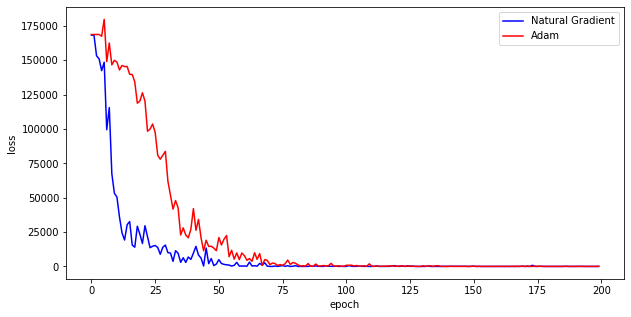
\includegraphics[width=0.4\textwidth]{images/vadam_compare.png}
\end{tabular}
\caption{The graph shows the loss versus epoch iteration of two optimization algorithm, Vadam and Adam. The blue is Vadam which uses natural gradient for update clearly converges to a loss quicker than Adam in red.}
    \label{fig:vadam_compare}
\end{figure}

We see from Figure \ref{fig:vadam_compare} that we get a quicker convergence by using natural gradient (blue) to train our model than using first-order method (red).

\section{Implementation and Results}
The implementation of the UDA code provided was rather straight forward.  The code was written in a recent python and used primarily a recent pytorch distribution.  A number of trivial modifications were made to support the most recent pytorch.

We adapted the UDA code-base by including calls to a natural gradient implementation sourced from github.  The code was well written, installed easily, and referenced by a couple modified calls in the existing UDA code-base. 

Initially we had some ambitious plans for a fine grained optimal hyper-parameter grid search over 8 Titan X GPUs using a parallel computing approach that would allow us to schedule GPUs resources for near optimal resource allocation. The UDA code base however makes frequent calls to pytorch routines that utilize multiprocessor options and managing this parallelism within a larger framework for parallelism was deemed beyond the scope of this report.  

Instead we hand balmed the jobs to the GPUs and ran less aggressive schedule for the grid search. 

All other things being equal   


\section{Discussion}
Note that Vadam works very well in this case because both Vadam and I have the same assumption about the form of variation distributions and its prior. Further, Vadam is developed exactly to adapt the Adam algorithm for variational inference through natural gradient.

Although we seen how using natural gradient helps us to achieve faster convergence rate, broader application of natural gradient descant for neural network training remains restricted by the problem domain. 
Another criticism of the use of natural gradient is that, it is unclear whether the faster convergence in epoch step is justified by the slow computation of FIM. 
% Further, there are first-order heuristics which approximates the Hessian of the loss which enables Newton method for optimization. 

\section{Conclusion}

In this report we introduced the unsupervised domain adaptation problem and leveraged variational inference technique to learn a prior distribution for domain adaptation.
In addition, we shown experimentally that using natural gradient results in quicker convergence in terms of epoch step for variational inference.

In conclusion, when the situation arises, we can consider using natural gradient for model training as it yields faster model convergence.
{\small
\bibliographystyle{ieee}
\bibliography{Fall2017_ProjectFinal_ProjectReportTemplate}
}

\section*{Appendix}

\subsection*{Team contributions}

\begin{description}
	
\end{description}

\end{document}

